\documentclass[android.tex]{subfiles}
\usepackage{subfiles}
\documentclass[12pt,oneside]{memoir} 
\usepackage[latinica]{matfmaster} 

\begin{document}

\begin{figure}[!ht]
  \centering
  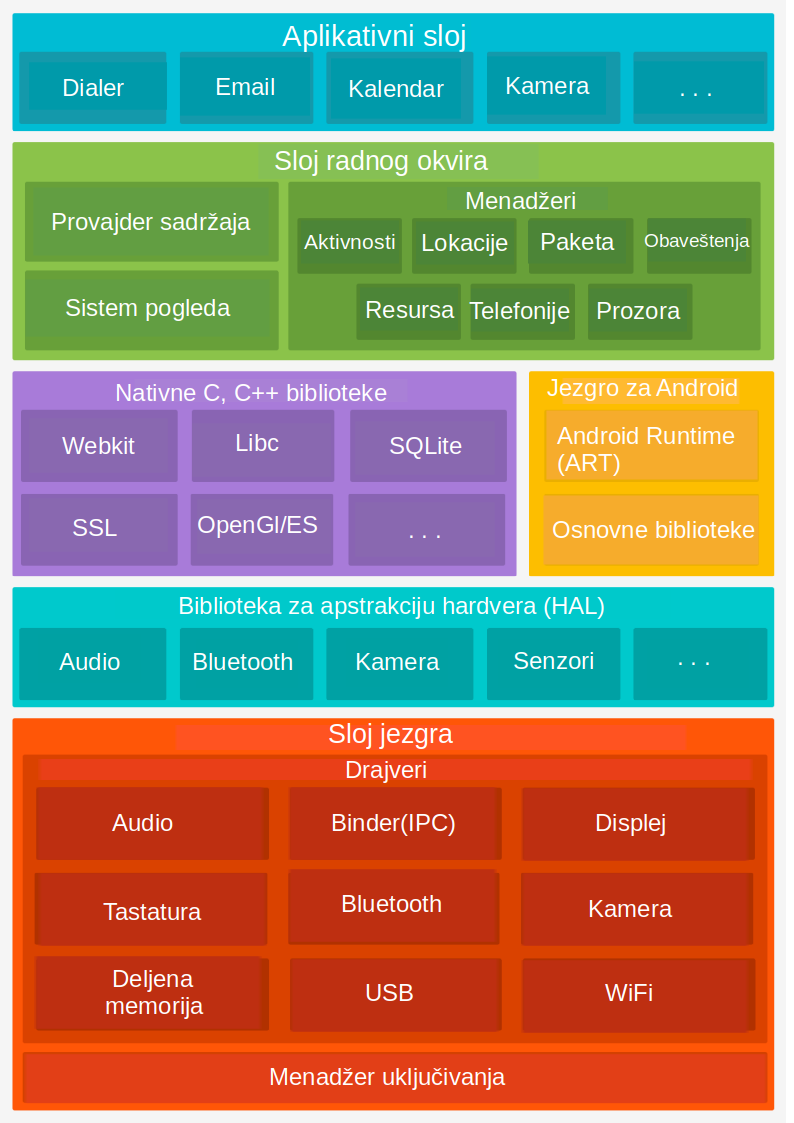
\includegraphics[width=0.9\textwidth]{arhitekturaSrp.png}
  \caption{Arhitektura OS Android, slika kreirana na osnovu \cite{sajt:androidDevelopersArhitektura}}
  \label{fig:arhitektura}
\end{figure}

Platforma Android predstavlja skup komponenti kao što su OS Android, biblioteke, radni okviri, API-ji i sl. koji omogućavaju razvoj i izvršavanje Android aplikacija. Zasnovana je na Linuks jezgru pri čemu se jezgro i drajveri nalaze u prostoru jezgra (eng. \textit{kernel space}), a nativne biblioteke u korisničkom prostoru (eng. \textit{user space}). Sve aplikacije se izvršavaju u Java virtuelnoj mašini koja se zove \textit{Android Runtime (ili, skraćeno, ART)}, a postoje Java biblioteke koje povezuju aplikaciju sa bibliotekama napisanim u nativnom jeziku. Sama arhitektura softvera kod Androida je slojevita i postoje četiri sloja koja se naslanjaju na sloj fizičke arhitekture. Slojevi arhitekture prikazani su na slici \ref{fig:arhitektura}, a navedeni od viših ka nižim (eng. \textit{top-down}) su \cite{book:papp}:
\begin{description}
\item \textbf{Aplikativni sloj} (eng. \textit{application layer}) predstavlja skup svih aplikacija koje se izvršavaju na Androidu. Aplikacije mogu biti sistemske, ugrađene ili korisničke. Sistemske su one koje je napisao proizvođač uređaja, ugrađene su one koje su drugi kreirali ali su unapred instalirane na uređaj i ne mogu se obrisati, a sve ostale su korisničke.
\item \textbf{Sloj radnog okvira} (eng. \textit{frameworks layer}) predstavlja sloj koji omogućava da se premoste razlike između aplikativnog i nativnog sloja i koji određuje ograničenja koja moraju da se poštuju pri razvoju Android aplikacija. Ovaj sloj je napisan u programskom jeziku Java, a pomoću interfejsa JNI (skraćeno od eng. \textit{Java Native Interface}) komunicira sa nativnim slojem. Najbitniji elementi sloja mogu se videti na slici \ref{fig:arhitektura}, a neki od njih su: menadžer aktivnosti koji upravlja životnim ciklusom aplikacije, menadžer paketa koji poseduje informacije o svim instaliranim aplikacijama na uređaju, menadžer lokacije koji pronalazi geografsku lokaciju uređaja i menadžer telefonije koji omogućava pristup sadržajima telefonije kao što su brojevi telefona. 
\item \textbf{Izvršni sloj} (eng. \textit{runtime layer}) napisan je u nativnom jeziku (C ili C++), sastoji se od nativnih biblioteka, biblioteka za apstrakciju hardvera (\textit{HAL}) i izvršnog okruženja za Android (eng. \textit{Android runtime}) u koji spadaju osnovne bibilioteke i ART. Do verzije 5.0 ART nije postojao već je korišćena \textit{Dalvik virtuelna mašina (skraćeno DVM)} \cite{sajt:dalvik}. 
\item \textbf{Sloj jezgra} (eng. \textit{kernel layer}) predstavlja sloj između hardvera i softvera koji poseduje sve drajvere koji su potrebni za hardverske komponente. Takođe, u ovom sloju je moguće pronaći sve vezano za upravljanje memorijom, procesima i uključivanjem, kao i o bezbednosti. 
\end{description}




\end{document}